\chapter[Datos]{Datos}
\label{Chap2}

Navarra dispone de dos confederaciones hidrográficas, la del cantábrico y la del ebro. Estas son organismos encargados de la gestión de cuencas hidrográficas que discurren por múltiples comunidades autónomas. Tomando como cuenca hidrográfica a la superficie por la cual fluye un conjunto de agua, como ríos, arroyos y lagos hasta su desembocadura en el mar.\newline
\newline
La del cantábrico ejerce sobre aquellos ríos cuya desembocadura va a parar al cantábrico, mientras, la del ebro trabaja sobre las zonas limitadas al cauce del ebro.\newline
\newline
No se hace uso de la página de la confederación del ebro al disponer de datos de otras páginas como la de la agencia estatal de meteorología y, la de agua en navarra. 

\begin{figure} [H]
	\centering
	\includegraphics[width=0.7\textwidth]{fig/ConfederacionesHidrográficas.jpg}
	\caption[Confederaciones hidrográficas en España]{Confederaciones hidrográficas en España}
	\label{fig:ej32}
\end{figure}

Creadas en 1926, las confederaciones son organismos autónomos, con plena autonomía funcional, adscritas al Ministerio para la Transición Ecológica y el Reto Demográfico. El papel desempeñado por estas recae entre otras cosas en, la planificación hidrológica, gestión de recursos y aprovechamientos, protección del dominio público hidráulico, control de calidad del agua y los bancos de datos.\newline
\newline
Por todo esto, es de gran importancia para este proyecto la adquisición de datos relacionados a estas entidades que ejercen en Navarra.

\section{CHCantábrico}
En la sección de nivel del río de la pagina de CHCantábrico, se encuentra la tabla con las estaciones, figura \ref{fig:sub9}. Una peculiaridad de esta, es que aun seguir una estructuración típica de tabla mediante el uso de \textit{table}, dispone de una tabla adicional en cada una de las filas. Figura \ref{fig:sub10}.

\begin{figure} [H]
	\centering
	\begin{subfigure}{.5\textwidth}
		\centering
		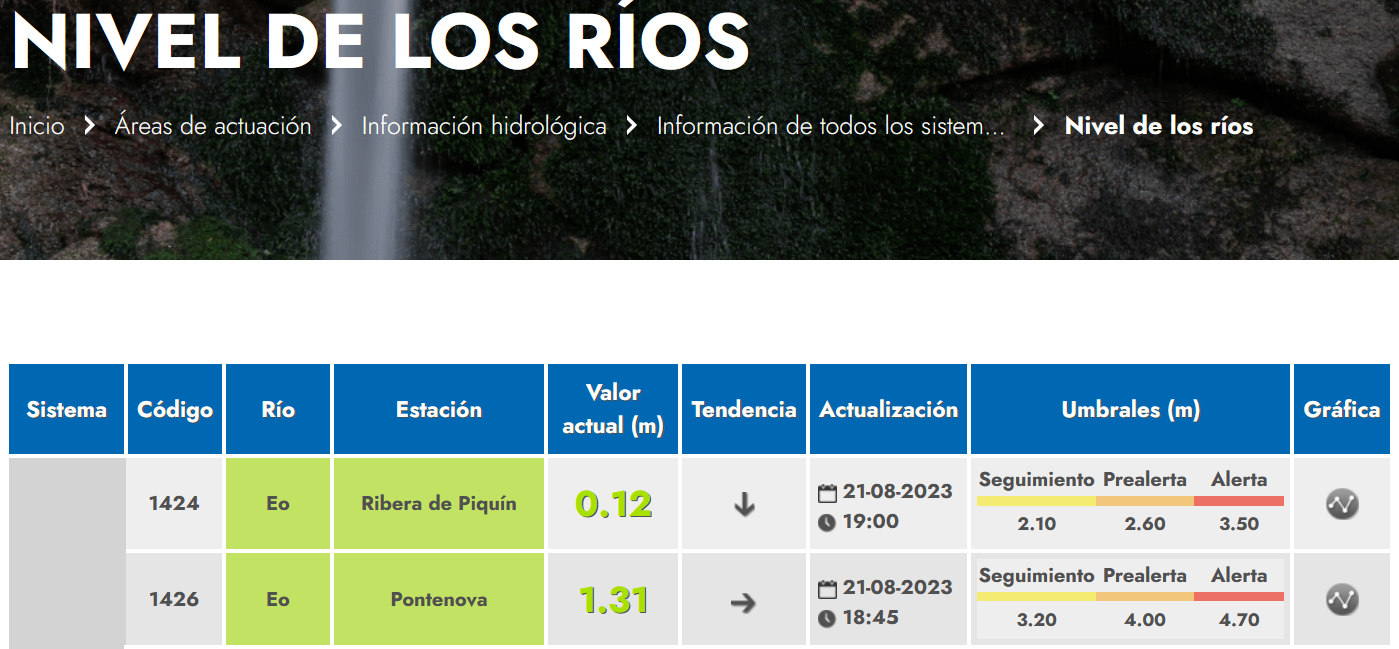
\includegraphics[width=.7\linewidth]{fig/CHCantabricoCode.png}
		\caption{Tabla estaciones}
		\label{fig:sub9}
	\end{subfigure}%
	\begin{subfigure}{.5\textwidth}
		\centering
		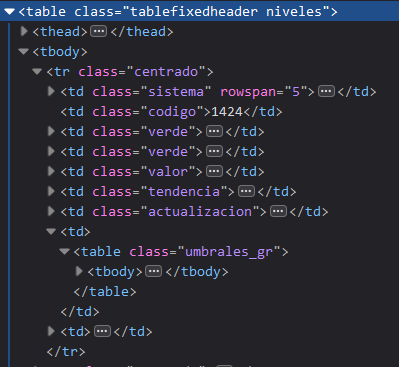
\includegraphics[width=.7\linewidth]{fig/CHCantabricoCodeHTML.png}
		\caption{HTML de la tabla de estaciones}
		\label{fig:sub10}
	\end{subfigure}
	\caption{Página Nivel de los ríos CHCantábrico}
	\label{fig:ej30}
\end{figure}

A diferencia del resto de las páginas visitadas, CHCantábrico no muestra los datos sobre la web, por el contrario, implementa un botón con el que descargarlos directamente en formato CSV. Los datos que se pueden obtener, son aquellos presentes en la tabla secundaria de las fila, los datos de pre-alerta, alerta y seguimiento para cada una de las estaciones, siendo datos valiosos a la hora de intentar anticipar inundaciones. Las coordenadas a su vez, tampoco vienen dados sobre la web, por lo que hace falta visitar la web del Centro de Estudios Hidrológicos (\url{https://ceh.cedex.es/}) para obtenerlas.

\section{Agencia estatal de Meteorología (Aemet)}
La figura \ref{fig:ej3} muestra la página web de Aemet, dentro podemos encontrar de forma accesible múltiples datos relacionados con la meteorología tomados cada hora, de los cuales seleccionaremos únicamente temperatura, precipitación y humedad, puesto que los datos relacionados con el viento no son tan relevantes para este proyecto. A su vez, no todas las estaciones muestran estos datos, ocurriendo lo mismo con los de presión atmosférica.

\begin{figure} [H]
	\centering
	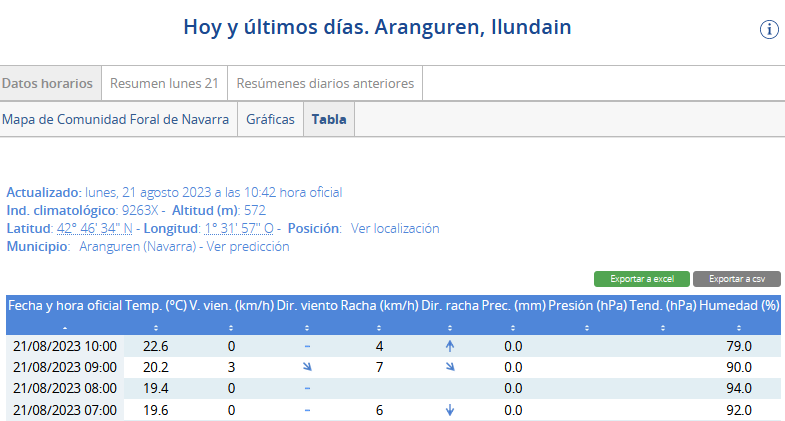
\includegraphics[width=0.7\textwidth]{fig/AemetData.png}
	\caption[Página Aemet de la estación en Aranguren (Navarra)]{Página Datos Aemet}
	\label{fig:ej3}
\end{figure}

Los datos en HTML vienen datos dentro de un elemento tabla, figura \ref{fig:ej20}, lo que facilita su adquisición, pues permite tomar todas las filas (elementos \textit{tr}) pertenecientes al elemento \textit{tbody} de esta. Una vez obtenidas las filas, la forma de lograr los datos deseados seria eligir dentro de cada elemento \textit{tr} los elementos \textit{td} deseados, puesto que HTML empieza a contar elementos desde el uno (en vez de cero como suele ser común en lenguajes de programación), los \textit{td} a obtener serian: uno, fecha y hora; dos, temperatura; siete, precipitación; diez, humedad.

\begin{figure} [H]
	\centering
	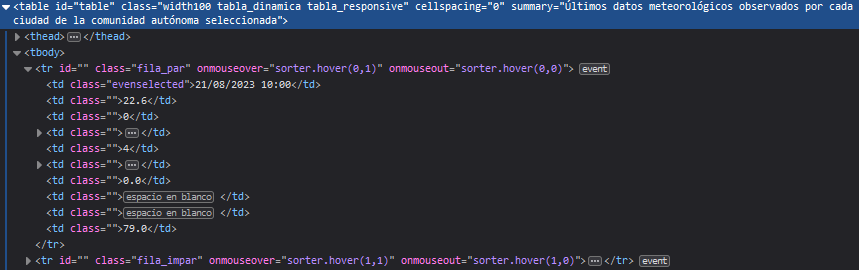
\includegraphics[width=0.7\textwidth]{fig/AemetDataHTML.png}
	\caption[HTML de la tabla de datos de Aemet de la estación en Aranguren (Navarra)]{HTML Tabla Datos Aemet}
	\label{fig:ej20}
\end{figure}

Las coordenadas, dentro de un \textit{span}, figura \ref{fig:ej21}, están incluidas en elementos \textit{abbr} con sus respectivas clases \textit{''latitude``} y \textit{''longitude``}, haciendo posible su obtención fácilmente mediante los elementos \textit{abbr}.

\begin{figure} [H]
	\centering
	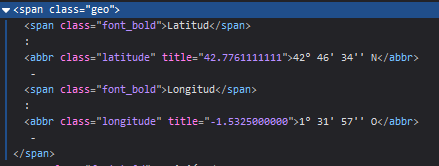
\includegraphics[width=0.7\textwidth]{fig/AemetCoordHTML.png}
	\caption[HTML de las coordenadas de Aemet de la estación en Aranguren (Navarra)]{HTML de las coordenadas en Aemet}
	\label{fig:ej21}
\end{figure}

\section{Meteorología y climatología de Navarra (MeteoNavarra)}
En la página de meteorología y climatología de Navarra encontramos una gran sección de estaciones de las cuales poder obtener datos. Figura \ref{fig:ej27}.

\begin{figure} [H]
	\centering
	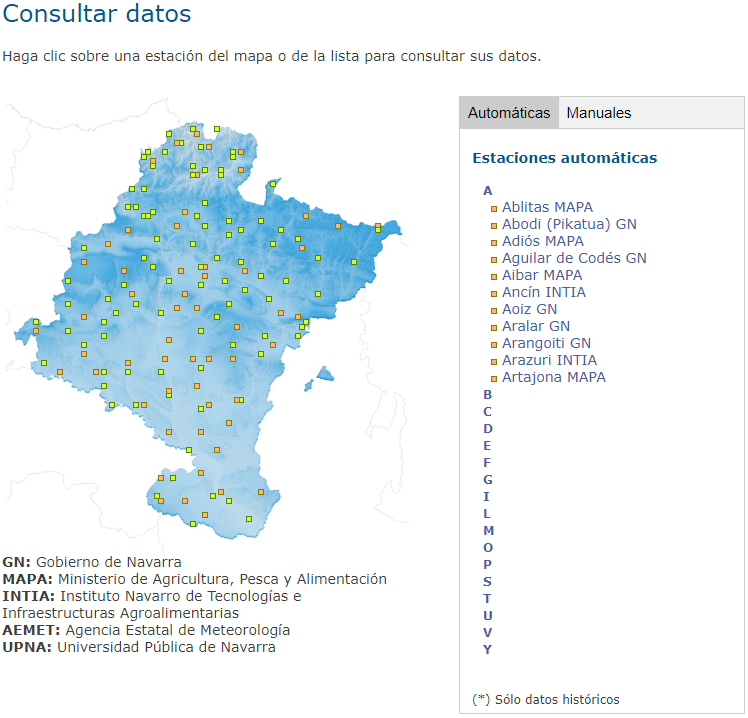
\includegraphics[width=0.7\textwidth]{fig/MeteoNavarraCode.png}
	\caption[Página estaciones MeteoNavarra]{Página estaciones MeteoNavarra}
	\label{fig:ej27}
\end{figure}

De entre los dos tipos e estaciones disponibles, automática y manual, únicamente se va a trabajar con los datos de las estaciones automáticas. El motivo de esto es que las manuales solo proveen datos diarios de, la temperatura máxima, mínima y de la precipitación acumulada. Esto hace que no se disponga de ningún dato hasta que finalice el día, cosa que no es viable si lo que se propone es predecir cambios radicales en un periodo de tiempo reducido.
\newline
\newline
Debido a la estructuración HTML usada para mostrar las estaciones, figura \ref{fig:sub5}, se puede ver que aun usar el elemento \textit{table}, este solo dispone de una única fila y columna, haciendo de la columna un elemento \textit{div} sobre el que insertar los datos, figura \ref{fig:sub6}. Como es el caso de la web de Agua en Navarra.

\begin{figure} [H]
	\centering
	\begin{subfigure}{.5\textwidth}
		\centering
		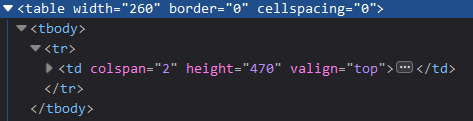
\includegraphics[width=.8\linewidth]{fig/MeteoNavarraCodeHTMLTable.png}
		\caption{Tabla}
		\label{fig:sub5}
	\end{subfigure}%
	\begin{subfigure}{.5\textwidth}
		\centering
		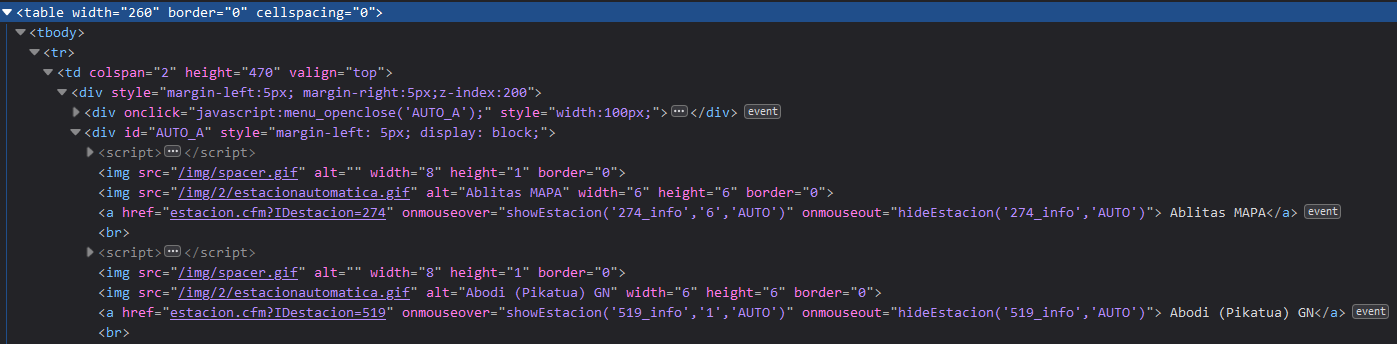
\includegraphics[width=.9\linewidth]{fig/MeteoNavarraCodeHTML.png}
		\caption{Filas}
		\label{fig:sub6}
	\end{subfigure}
	\caption{HTML tabla estaciones MeteoNavarra}
	\label{fig:ej28}
\end{figure}

Las estaciones automáticas proporcionan tanto datos en periodos de diez minutos como datos diarios. Tras usar el mismo razonamiento que con las estaciones manuales, no tomamos los datos diarios y, entre los actualizados cada diez minutos, se toman la temperatura, humedad relativa, radiación global y precipitación. El resto se omitirán. Figura \ref{fig:ej6}.

\begin{figure} [H]
	\centering
	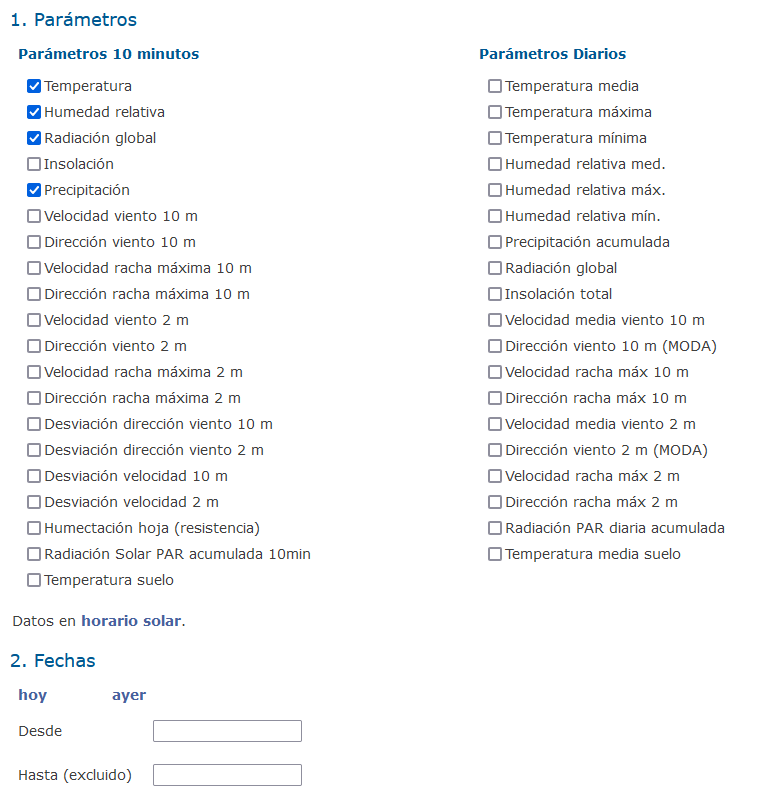
\includegraphics[width=0.6\textwidth]{fig/DatosMeteoNavarra.png}
	\caption[Apartado selección de datos MeteoNavarra]{Datos MeteoNavarra}
	\label{fig:ej6}
\end{figure}

Los datos se muestran en formato tabla, tanto visualmente, en la figura \ref{fig:sub7} como a nivel de HTML, figura \ref{fig:sub8}, cosa que facilita su obtención.

\begin{figure} [H]
	\centering
	\begin{subfigure}{.5\textwidth}
		\centering
		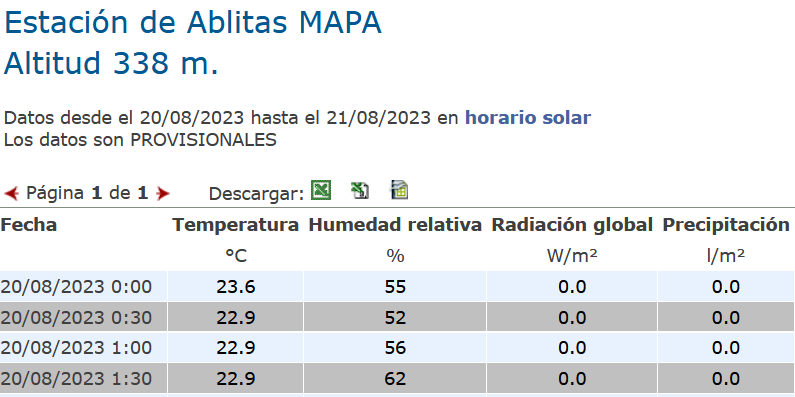
\includegraphics[width=.7\linewidth]{fig/MeteoNavarraData.png}
		\caption{Tabla datos}
		\label{fig:sub7}
	\end{subfigure}%
	\begin{subfigure}{.5\textwidth}
		\centering
		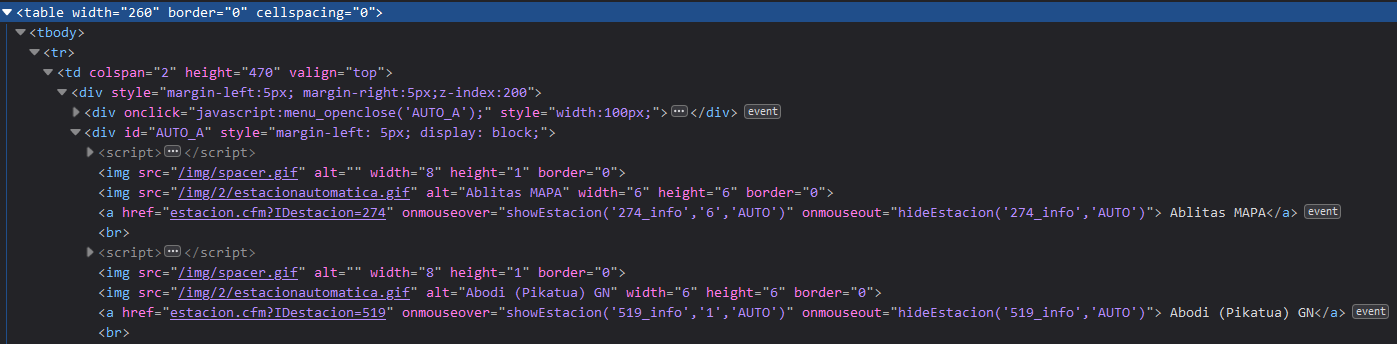
\includegraphics[width=.7\linewidth]{fig/MeteoNavarraCodeHTML.png}
		\caption{HTML de la tabla de datos}
		\label{fig:sub8}
	\end{subfigure}
	\caption{Página de datos de MeteoNavarra}
	\label{fig:ej29}
\end{figure}

\section{El Agua en Navarra}
En esta página encontraremos los datos tanto del nivel de los ríos como de su caudal en los últimos 15 días en periodos de 10 minutos, siendo una de las fuentes principales de datos.
\newline
\newline
La sección de aforos en la página, figura \ref{fig:ej4}, muestra el mapa de Navarra junto a varias estaciones. Aunque no todas las disponibles en la web, conformando unicamente el grupo de estaciones principales.\newline
\newline
Con el fin de acceder a todas las estaciones disponibles, debemos centrarnos en el mapa de la esquina inferior derecha. Estructurada en 6 regiones, Norte, Arga, Ega, Ebro alto, Ebro bajo y Aragón, por medio de este mapa accedemos a cada región, mostrando el mapa de la región, dando acceso a todas las estaciones en la zona.

\begin{figure} [H]
	\centering
	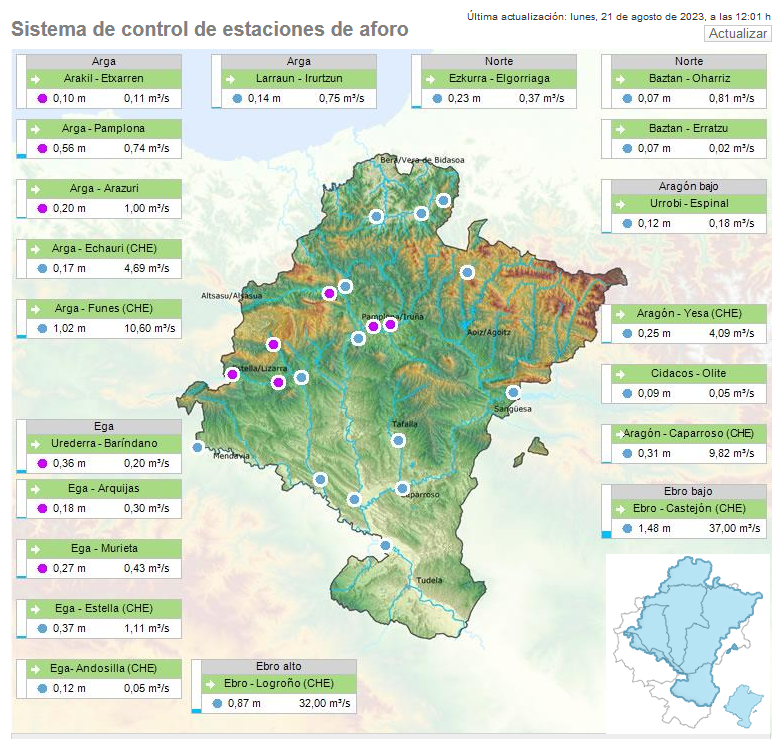
\includegraphics[width=0.7\textwidth]{fig/AguaEnNavarraCode.png}
	\caption[Página principal de aforos de El Agua en Navarra]{Página El Agua en Navarra}
	\label{fig:ej4}
\end{figure}

El HTML del mapa se estructura de la siguiente manera, figura \ref{fig:ej22}, mostrando un par de elementos \textit{area} por estación, uno con \textit{shape=''rect``}, representando las tarjetas que rodean el mapa y otro con \textit{shape=''circle``}, siendo los puntos en el mapa. Pulsar sobre cualquiera de ellos es equivalente, aunque posteriormente hagamos uso de los elementos con \textit{shape=''rect``} dentro del código.

\begin{figure} [H]
	\centering
	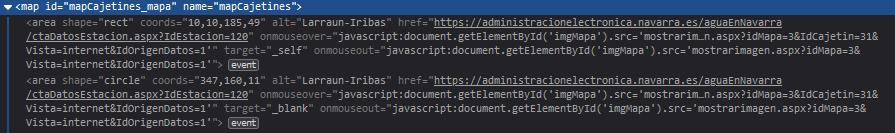
\includegraphics[width=0.7\textwidth]{fig/AguaEnNavarraCodeHTML.png}
	\caption[HTML mapa estaciones de El Agua en Navarra]{HTML mapa estaciones El Agua en Navarra}
	\label{fig:ej22}
\end{figure}

Las paginas de cada estación se muestran como en la figura \ref{fig:ej23}.

\begin{figure} [H]
	\centering
	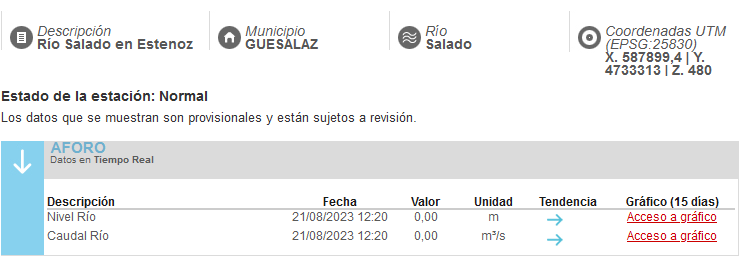
\includegraphics[width=0.7\textwidth]{fig/AguaEnNavarraEstacion.png}
	\caption[Página estación de El Agua en Navarra]{Página estación El Agua en Navarra}
	\label{fig:ej23}
\end{figure}

De ella obtenemos los próximos datos, descripción, municipio, río y coordenadas. Ademas de darnos acceso a los datos de nivel y caudal del río. Mostrados dentro de el \textit{div} con \textit{id=''blog\_icons``}, figura \ref{fig:ej24}. Una vez dentro del \textit{div} todos los datos siguen la misma estructuración, \textit{''//div/span/span``}, permitiendo la adquisición de todos los elementos a la vez.

\begin{figure} [H]
	\centering
	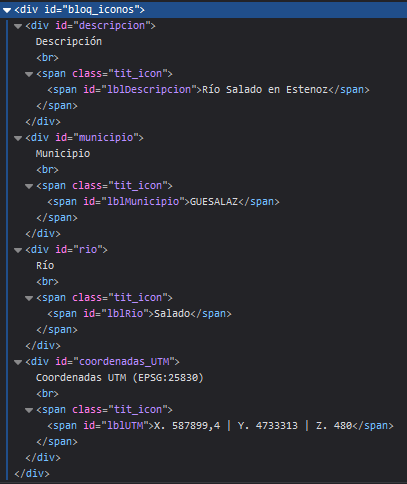
\includegraphics[width=0.5\textwidth]{fig/AguaEnNavarraEstacionHTML.png}
	\caption[HTML estación de El Agua en Navarra]{HTML estación El Agua en Navarra}
	\label{fig:ej24}
\end{figure}

Una vez se accede a los datos de la estación, se mostrara una gráfica como la de la figura \ref{fig:ej25}. A su vez, mediante el botón \textit{''Datos Numéricos``}, tendremos la posibilidad de observar los datos en forma numérica. Pero no sin antes haber visitado la versión gráfica. Pues da el error de la figura \ref{fig:ej5}.

\begin{figure} [H]
	\centering
	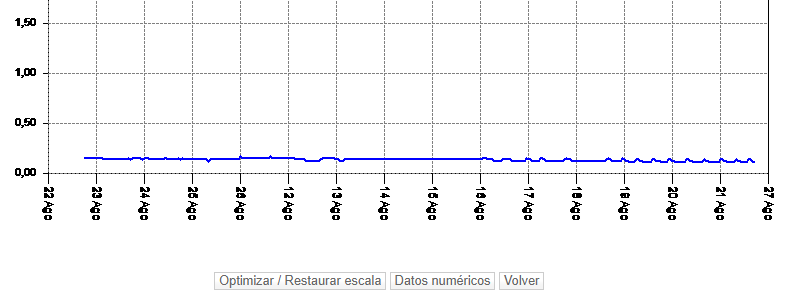
\includegraphics[width=0.7\textwidth]{fig/AguaEnNavarraGrafica.png}
	\caption[Gráfica de datos en estación de El Agua en Navarra]{Gráfica datos estación El Agua en Navarra}
	\label{fig:ej25}
\end{figure}

\begin{figure} [H]
	\centering
	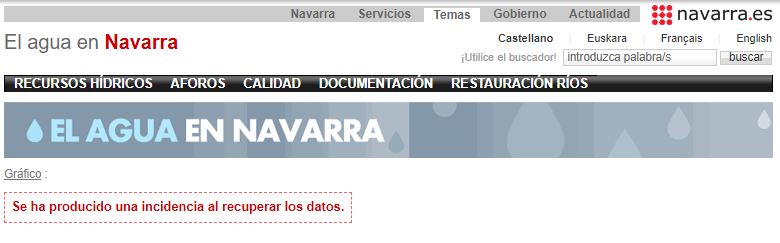
\includegraphics[width=0.7\textwidth]{fig/ErrorAguaEnNavarra.png}
	\caption[Error al cargar directamente la página de datos numéricos en El Agua en Navarra]{Error datos numéricos en El Agua en Navarra}
	\label{fig:ej5}
\end{figure}

Los datos numéricos están presentados en formato tabla como se aprecia en la figura \ref{fig:sub3}. Por el contrario, tras observar el HTML, realmente es un elemento \textit{div}, que engloba los conjuntos de elementos \textit{span} que representan las lineas, separados por elementos br, figura \ref{fig:sub4}. El formato en el que se presentan los datos, no hace más que representar una mayor complejidad para, posteriormente, trabajar y adquirir los datos. 

\begin{figure} [H]
	\centering
	\begin{subfigure}{.5\textwidth}
		\centering
		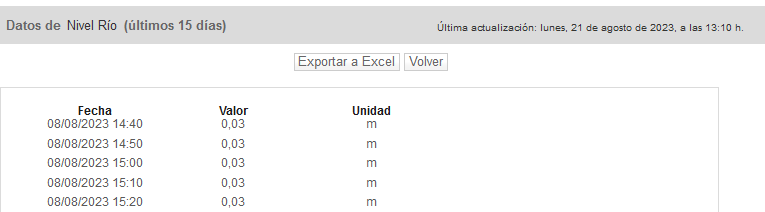
\includegraphics[width=.9\linewidth]{fig/AguaEnNavarraData.png}
		\caption{Formato presentación de los datos}
		\label{fig:sub3}
	\end{subfigure}%
	\begin{subfigure}{.5\textwidth}
		\centering
		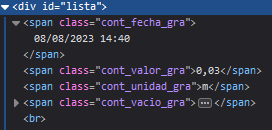
\includegraphics[width=.7\linewidth]{fig/AguaEnNavarraDataHTML.png}
		\caption{HTML de los datos}
		\label{fig:sub4}
	\end{subfigure}
	\caption{Datos numéricos de estaciones en Agua en Navarra}
	\label{fig:ej26}
\end{figure}

De las webs mencionadas se dispone de los siguientes datos para este proyecto:

\begin{itemize}
	\setlength\itemsep{0.5em}
	\item Nivel (m)
	\item Caudal ($m^3/s$)
	\item Precipitación (mm)
	\item Temperatura (ºC)
	\item Humedad (\%)
	\item Radiación ($W/m^2$)
\end{itemize}

A su vez, se dispone de la fecha y hora en la que se hizo la lectura de los datos, junto con los códigos y coordenadas de las estaciones sobre las cuales se obtienen los datos.